\section{The ZX Spectrum}
The ZX Spectrum is an 8-bit generation personal computer released by Sinclair Research Ltd. It was first launched in the United Kingdom in 23rd April 1982 and discontinued in 1992. The ZX Spectrum was released as eight different models, from the 16KB RAM released in 1982 to the ZX Spectrum +3, released in 1987, with 128KB RAM and built in floppy disk drive. Like the Commodore 64, the ZX Spectrum was among the first mainstream audience home computers.

\subsection{System architecture}
The ZX Spectrum is based on a 3.54MHz Zilog Z80A CPU connected to a ULA responsible for all the interfaces (tape, sound, keyboard and video) and to an arrangement of three input/output buses. These buses are the Data Bus, the Address Bus and Control Bus. The CPU can address up to 64KB of memory. The first model came with a 16KB RAM followed by a 48KB RAM version and later by 128KB RAM versions. The ULA is able to bring the CPU to a temporary halt, giving it absolute priority and allowing it to access the standard RAM without interference from the CPU. The video output is through a RF modulator and has a 32x22 character text display with 256x192 pixel resolution and 8 colors. The sound in the 16/48KB models has one beeper capable of producing 1 channel with 5 octaves, the 128KB model was capable of producing 3 channels with 5 octaves.
A T-state is the equivalent to the time length of one clock pulse to the CPU, in the case of the Z80, one T-state has the duration of 1/3500000 seconds. The T-states are used for synchronizing the rendering of screen lines that make one frame. In the 48K version there are 224 T-states/screen line (scanline) and 312 screen lines/frame. In the 128K version the number of T-states/screen line increases for 228 and the number of screen lines/frame decreases for 63.
This CPU was an improvement to the 8080 with instruction set capable of performing bit manipulation, block move and block I/O, new index registers with instructions for direct base+offset addressing and a better interrupt system. Like on the 8080 the 8-bit registers are typically coupled to provide a 16-bit version.

\begin{figure}
	\center{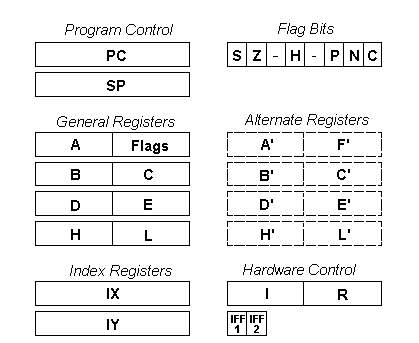
\includegraphics[width=0.4\textwidth]{img/z80_reg.png}}
	\caption{Z80 CPU registers.}
\end{figure}

Z80 instructions are represent in memory as byte sequences with following forms:
\begin{itemize}
\item {[prefix byte,]  opcode  [,displacement byte]  [,immediate data]}
\item {two prefix bytes,  displacement byte,  opcode}
\end{itemize}
The Z80 uses 252 codes as single byte opcodes (no prefix byte), the remaining four are used as opcodes prefixes: CBh and EDh enable extra instructions, DDh or FDh selects IX+displacement or IY+displacement. This are useful to access data organized in fixed structures but tend to be slower than using sequences of using HL register and increment it.
The Z80 instructions are grouped into the following categories:
\begin{itemize}
\item {8-bit arithmetic and logic operations}
\item {16-bit arithmetic}
\item {8-bit load}
\item {16-bit load}
\item {Bit set, reset, and test}
\item {Call, return, and restart}
\item {Exchange, block transfer, and search}
\item {General purpose arithmetic and CPU control}
\item {Input and output}
\item {Jump}
\item {Rotate and shift}
\end{itemize}
Z80 doesn’t have any multiply instruction available.

\subsection{Memory architecture}
The Z80 processor is a 8-bit CPU,but can operate 8-bit or 16-bit values, that allows index up to 64K of memory. The 48K Spectrum has 16K ROM and 48K RAM, meaning that the processor indexes directly  the memory. For the 128 and +2 Spectrums, there are two 16K pages of ROM and eight 16K pages of RAM. For the +3, +2A, +2B Spectrums there are twelve 16K pages, four pages for ROM and eight pages for RAM. From this ten and twelve pages, only four are visible to the CPU.
The CPU addressable memory, from 0 (0000h) to 65535 (FFFFh) is slitted in four 16K areas. The lower 16K bytes of memory (0000h-3FFFh) are the ROM which holds the monitor program, divided between the input/output routines, the BASIC interpreter and expression handler. The next 16K bytes (4000h-7FFFh) are RAM used to hold the system variables, buffers and screen area. The last 32K (8000h-FFFFh) are RAM that provides extra memory space for the user.
In the 128K versions, when the system boots, it maps the ROM 0 to the 0000h-3FFFh addresses, RAM 5 to 4000h-7FFFh addresses and RAM 2 and RAM 0 to 8000h-BFFFh and C000h-FFFFh addresses respectively. All the hidden memory becomes visible to the hardware using a method called paging.

\subsection{Paging}
We can send a combination of bits to an I/O port to select which memory page we want to use. The I/O address used to select the RAM page is at 32765 (7FFDh) address and accepts a 6-bit long number. Each bit in this number has its function, Bit 0 to Bit 2 selects which RAM page (0-7) goes to the highest seen addresses of the memory (C000h-FFFFh). Bit 3 switches screens. There is two RAM pages in memory that can hold a screen, RAM 5 (screen 0) and RAM 7 (screen 1). This operation does not change the content of RAM 5 which is always paged between 4000h and 7FFFh. Bit 4 selects which ROM is paged into lower addresses of the memory (0000h-3FFFh). For the Spectrum version with four ROM pages, this bit is used in combination with bit 2 of port 1FFDh. In the versions of Spectrum with two ROMs, ROM 0 contains the 128K editor and menu, ROM 1 contains the 48K BASIC. For the versions with four ROMs, ROM 0 contains the 128K editor, ROM 1 contains the 128K syntax checker, ROM 2 contains +3DOS and ROM 3 contains the 48K BASC. Bit 5 function is to disable paging operations, if this bit is set, paging operations will no longer work and the machine will assume the 48K configuration. To turn the machine back to the 128K configuration, this must be switched off or reseted.
From the +3 and followings, the I/O port 1FFDh is used for ROM and RAM switching with a 5-bit long number. Bits 0 and 1 are used for ROM/RAM switching, the value in bit 2 affects how bits 0 and 1 work in RAM/ROM switching operations. Bit 3 is related with the disk motor and bit 4 with the printer strobe.
When bit 0 is 0 in port 1FFDh, combining bit 4 in port 7FFDh and bit 2 in port 1FFDh we can form a 2-bit number, bit 4 is the least significant bit and bit 2 the most significant bit, which decides which ROM is paged to lowest memory addresses (0000h-3FFFh).
\begin{table}[h]
\centering
	\begin{tabular}{|{c}|{c}|{c}|}
	\hline
	& Bit 2 1FFDh & Bit 4 7FFDh \\ \hline
	ROM 0 & 0 & 0 \\ \hline
	ROM 1 & 0 & 1 \\ \hline
	ROM 2 & 1 & 0 \\ \hline
	ROM 3 & 1 & 1 \\ \hline
\end{tabular}
\caption{ROM switching}
\end{table}

When bit 0 in port 1FFDh has the value 1, bits 1 and 2 are used to perform a special paging mode in which all four pages in memory contain RAM. These are the possible combinations:
\begin{table}[h]
\centering
\begin{tabular}{|{c}|{c}|{c}|}
	\hline
	& Bit 2 1FFDh & Bit 1 1FFDh \\ \hline
	Mode 0 & 0 & 0 \\ \hline
	Mode 1 & 0 & 1 \\ \hline
	Mode 2 & 1 & 0 \\ \hline
	Mode 3 & 1 & 1 \\ \hline
\end{tabular}
\caption{Bit combination}
\end{table}
\begin{table}[h]
\centering
\begin{tabular}{|p{1,2cm}|{c}|{c}|{c}|{c}|}
 \hline
	& Mode 0 & Mode 1 & Mode 2 & Mode 3 \\ \hline
	0xFFFFh - 0xC000h & RAM 3 & RAM 7 & RAM 3 & RAM 3 \\ \hline
	0xBFFFh - 0x8000h & RAM 2 & RAM 6 & RAM 6 & RAM 6 \\ \hline
	0x7FFFh - 0x4000h & RAM 1 & RAM 5 & RAM 5 & RAM 7 \\ \hline
	0x3FFFh - 0x0000h & RAM 3 & RAM 4 & RAM 4 & RAM 4 \\ \hline
\end{tabular}
\caption{Extended memory paging}
\end{table}